% Current scope: frozen v1, moderate synthetic OCR only.
\documentclass[11pt]{article}
\usepackage[review]{acl}
\usepackage{times}
\usepackage{latexsym}
\usepackage[T1]{fontenc}
\usepackage[utf8]{inputenc}
\usepackage{microtype}
\usepackage{inconsolata}
\usepackage{graphicx}
\usepackage{booktabs}
\usepackage{amsmath}
\usepackage{amssymb}
% GENERATED from pinned v1 artifacts.
\newcommand{\ExactFone}{0.269 [0.249, 0.288]}
\newcommand{\ExactWrongName}{150}
\newcommand{\RuleFone}{0.606 [0.569, 0.645]}
\newcommand{\RuleWrongName}{147}
\newcommand{\LocalFone}{0.981 [0.974, 0.989]}
\newcommand{\LocalWrongName}{144}
\newcommand{\ArchiveFone}{0.844 [0.827, 0.862]}
\newcommand{\ArchiveWrongName}{8}
\newcommand{\RuleReview}{93.05}
\newcommand{\RuleRisk}{0.00}
\newcommand{\LocalReview}{28.57}
\newcommand{\LocalRisk}{2.67}
\newcommand{\ArchiveReview}{57.24}
\newcommand{\ArchiveRisk}{5.57}
\newcommand{\ReviewSaving}{64.48 [62.09, 66.76]}
\newcommand{\PilotCases}{60}
\newcommand{\PilotCandidates}{57}
\newcommand{\PilotUnresolved}{3}
\newcommand{\PilotDisputes}{1}

\title{KYC-NLI: Auditing Document-Level Inference and Selective Prediction
under Synthetic Cross-Script OCR Noise}
\author{Anonymous submission}
\begin{document}
\maketitle
\begin{abstract}
Checking a document against an identity claim requires distinguishing supporting,
refuting and missing evidence. We study this distinction using KYC-NLI, a
synthetic diagnostic benchmark across five scripts, and a corrected, frozen
version containing 7,000 instances split by identity. We evaluate string
matching, a transliteration-aware rule engine and two separately identified
recovered XLM-R checkpoints. On the 1,050-case moderate-noise test set, local
XLM-R obtains macro-F1 \LocalFone{}; archived XLM-R obtains \ArchiveFone{}.
At a common requested 5\% automation-error budget, development-selected policies
review \LocalReview\% of test cases for local XLM-R and \RuleReview\% for rules.
Their observed automation errors are \LocalRisk\% and \RuleRisk\%, respectively;
both meet the empirical target, without a population-risk guarantee. A
60-case human pilot yields 57 candidate human labels, three unresolved cases
and one retained human--generator disagreement. These findings support a
traceable diagnostic comparison while exposing label and provenance limitations;
they do not establish production verification accuracy.
\end{abstract}

\section{Introduction}
Identity verification involves a claim about a field and potentially several
noisy observations of that field. A spelling mismatch can reflect a different
value, a romanisation alternative, or damaged evidence. We formulate this task
as document-level natural language inference (NLI): entailment, contradiction
or neutral. Neutral denotes insufficient evidence, rather than personal or
model uncertainty. A neutral prediction is routed to human review; uncertain
entailment or contradiction predictions may also be deferred.

Our synthetic multi-zone document representation spans Latin, Devanagari,
Tamil, Bengali and Perso-Arabic scripts. It is inspired by identity-document
verification, but does not assert that Indian passports universally print
names in regional scripts. The machine-readable-zone (MRZ) layout is motivated
by the TD3 specification \citep{icao9303}; regional observations and temporal
validity constraints are synthetic design choices, not a certification of
compliance with issuing rules.

The contribution is a diagnostic evaluation, not a new neural architecture.
We provide a corrected benchmark version with an integrity audit, separate
checkpoint-specific results, and a review-load comparison at development-selected
error budgets. A human pilot tests whether generated labels survive textual
interpretation. It identifies ambiguities that high model scores alone conceal.

\section{Related Work}
Sentence-level NLI resources include SNLI and MultiNLI
\citep{bowman2015snli,williams2018mnli}. DocNLI extends premises to documents
\citep{yin2021docnli}; ContractNLI connects document-level decisions with evidence
\citep{koreeda2021contractnli}. Our premises are field observations rather than
continuous prose. Annotation artifacts and heuristic solutions can undermine
NLI evaluation \citep{gururangan2018annotation,mccoy2019right}; contrast sets
probe local decision boundaries \citep{gardner2020contrast}. We retain related
instances in contrast groups and keep entire identities in one split.

Dakshina provides human-elicited South Asian romanisations
\citep{roark2020dakshina}; this motivates matching beyond literal equality,
without validating every variant our generator produces. MIDV-2020 studies
identity-document analysis using mock documents \citep{bulatov2021midv2020}.
We evaluate synthetic field observations, not that image benchmark. Selective
classification evaluates prediction together with rejection
\citep{elyaniv2010foundations,geifman2017selective}; we distinguish error among
automated decisions from the fraction requiring human review.

\section{Benchmark and Integrity Audit}
An instance contains observations $P$, a field claim $h$, and generator label
$y\in\{E,C,N\}$. Observations identify a field, zone, script, observed value
and confidence. Entailment allows accepted romanisations and recoverable
corruption. Contradiction includes direct conflicts and constructed inconsistent
dates. Neutral instances remove a field or destroy its available evidence.
Unresolved human annotation is a separate status, never automatically neutral.

\paragraph{Frozen v1.}
Generation uses 200 fabricated identities per configured language and seed
20260906. Each identity produces seven instances. Table~\ref{tab:data} gives
the identity-disjoint splits; zero identity and contrast-group overlap is
asserted. No real identity record is an input. Names come from embedded
synthetic pools. Pool and engine equivalence checks do not establish the
linguistic validity of all alternative spellings.
\begin{table}[t]
\centering\small% GENERATED by scripts/make_tables.py -- do not edit by hand.
% Regenerate the result, then re-run the script.
\begin{tabular}{lrrrrrr}
\toprule
Split & Identities & Groups & Instances & E & C & N \\
\midrule
Train & 700 & 2100 & 4,900 & 1,400 & 2,100 & 1,400 \\
Dev & 150 & 450 & 1,050 & 300 & 450 & 300 \\
Test & 150 & 450 & 1,050 & 300 & 450 & 300 \\
\midrule
Total & 1000 & 3,000 & 7,000 & 2,000 & 3,000 & 2,000 \\
\bottomrule
\end{tabular}

\caption{Frozen v1 splits. E, C and N are generator labels.}\label{tab:data}
\end{table}

The audit found surname negatives that were accepted aliases of the same
native surname. The corrected generator excludes clean native forms, canonical
Latin forms, engine variants and pool aliases from negative sampling. It repairs
56 claims, including six in test. A separate deterministic random stream
preserves identity generation and OCR draws. Premises, split membership and
label counts stay fixed; repaired hypotheses, rationales and version provenance
change. This targeted repair is not comprehensive validation of the label function.

\paragraph{Noise scope.}
All current comparisons use frozen moderate noise. The simulator was calibrated
using Tesseract \citep{smith2007tesseract} on shaped, rendered text with simulated
degradation. This motivates the simulator but does not establish equivalence
to photographed documents or a lower bound on real-world error. Historical v0
noise sweeps are excluded. We make no clean-to-heavy generalization claim for
these checkpoints on corrected v1.

\section{Systems and Checkpoint Provenance}
\paragraph{Baselines.}
Exact matching compares normalized observed strings and never predicts neutral.
Rules combine configured transliteration variants, fuzzy matching, date parsing
and temporal constraints. Their matching thresholds and handling of missing
evidence are unchanged. The models do not receive the variant sets available
to rules. Some handwritten transliteration entries remain marked unverified
in source; we do not claim comprehensive standards validation.

\paragraph{Separate recovered artifacts.}
Both checkpoints have saved architecture
\texttt{XLMRobertaForSequenceClassification}, with the base configuration of
XLM-R \citep{conneau2020xlmr}. They are not DistilBERT models. We call them
\emph{local} and \emph{archived} by provenance, not performance. Weight hashes
differ; tokenizer files match. Both are reported rather than choosing the
better historical score. Table~\ref{tab:hashes} identifies them.

Saved training summaries describe XLM-R-base fine-tuning on v0 for four epochs,
learning rate $2\times10^{-5}$, batch size 32, unfrozen embeddings and seed
20260906. These are metadata declarations, not a reconstruction of original
execution or proof of original training-input bytes. The artifacts are not
controlled independent-seed replicates. Neither is retrained on v1. The held-out
identities do not overlap the preserved v0 training reference; this does not
independently certify an unavailable historical training run.

\paragraph{Inference.}
Input contains observed fields and the claim. Values below the shared
legibility threshold receive an unreadable marker. Clean pre-corruption values
and variant sets never enter model input. Both checkpoints use maximum length
192, batch size 4, CPU float32, two threads and deterministic evaluation.
The project mapping is 0=entailment, 1=contradiction, 2=neutral; saved
configurations themselves use generic label names. Tokenizer, weights, data,
code snapshot and inference settings are recorded for each run.

\section{Evaluation Protocol}
Classification is scored against frozen generator labels, using macro-F1,
class-wise F1, per-language macro-F1, phenomenon accuracy and contrast-group
consistency. Each macro-F1 has a 95\% percentile bootstrap interval from 1,000
contrast-group resamples. Paired comparisons resample the same groups for both
systems, following the rationale of paired resampling \citep{koehn2004significance}.
Intervals condition on recovered weights and data, not training-seed variability.

\paragraph{Selective policies.}
Predicted neutral always requires review. Otherwise a decision is automated
only if confidence is at least $t$. Automation error is wrong automated
decisions divided by all automated decisions. Review load is the fraction not
automated. A policy automating no cases has undefined risk, not zero risk.
For each budget, development data select the greatest automation satisfying the
empirical error cap, searching distinct confidence values and preserving ties.
Thresholds are recorded before the policy evaluator reads test predictions.
However, earlier test classification results had already been inspected: this
is retrospective development-selected analysis, not a new prospectively blinded
test. No test-tuned threshold is substituted for the locked policy.

Test uncertainty uses 1,000 contrast-group resamples with development thresholds
fixed. It excludes threshold-selection and training uncertainty. A common
requested budget does not mean equal realized test error; we report both.

\section{Results}
\subsection{Classification against Frozen Labels}
Table~\ref{tab:main} and Figure~\ref{fig:f1} report the independently evaluated
artifacts. Local XLM-R obtains \LocalFone{}, archived XLM-R \ArchiveFone{},
rules \RuleFone{} and exact matching \ExactFone{}.
Paired differences against rules (Table~\ref{tab:paired}) support a difference
on this synthetic test, not on real customer traffic.
\begin{table*}[t]
\centering\small% GENERATED by kyc-nli paper-v1; do not hand-edit.
\begin{tabular}{llrr}
\toprule
System & Macro-F1 [95\% CI] & Group & Name C \\
\midrule
Exact match & 0.269 [0.249, 0.288] & 0.000 & 150/150 \\
Rules & 0.606 [0.569, 0.645] & 0.316 & 147/150 \\
Local XLM-R & 0.981 [0.974, 0.989] & 0.956 & 144/150 \\
Archived XLM-R & 0.844 [0.827, 0.862] & 0.620 & 8/150 \\
\bottomrule
\end{tabular}

\caption{Frozen v1 test classification. Group is contrast-group consistency;
Name C is correct surname contradictions out of 150. Intervals resample contrast
groups. Scores use generator labels, not pilot replacements.}\label{tab:main}
\end{table*}
\begin{figure}[t]
\centering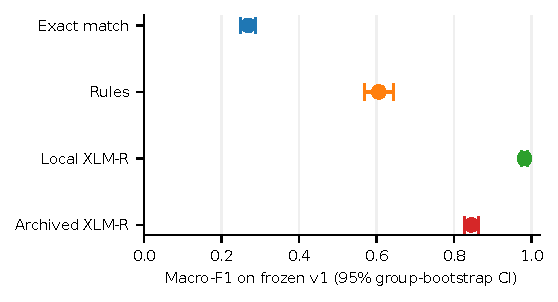
\includegraphics[width=\columnwidth]{figures/v1_classification}
\caption{Classification with 95\% contrast-group bootstrap intervals.}\label{fig:f1}
\end{figure}
Local XLM-R correctly labels \LocalWrongName{}/150 surname contradictions,
versus \ArchiveWrongName{}/150 for archived XLM-R. This disparity explains why
checkpoint identity matters to conflicting earlier reports. It does not identify
a causal training difference. Appendix tables give class, language and
phenomenon results.

\subsection{Review Load at a Requested Error Budget}
\begin{table*}[t]
\centering\small\resizebox{\textwidth}{!}{% GENERATED by kyc-nli paper-v1; do not hand-edit.
\begin{tabular}{lrlllc}
\toprule
System & Threshold & Review \% [95\% CI] & Errors/auto & Error \% [95\% CI] & Meets \\
\midrule
Rules & 1.000000 & 93.05 [91.63, 94.54] & 0/73 & 0.00 [0.00, 0.00] & Yes \\
Local XLM-R & 0.505705 & 28.57 [26.97, 30.21] & 20/750 & 2.67 [1.59, 3.73] & Yes \\
Archived XLM-R & 0.642608 & 57.24 [53.76, 60.86] & 25/449 & 5.57 [3.49, 7.57] & No \\
\bottomrule
\end{tabular}
}
\caption{Development-selected policies for a requested 5\% automation-error
budget applied unchanged to test. Meets refers to the point estimate only.
Brackets are conditional 95\% group-bootstrap intervals.}\label{tab:policy}
\end{table*}
Both local XLM-R and rules meet the empirical test target. Rules review
\RuleReview\% and make no observed errors among 73 automated decisions.
Local XLM-R reviews \LocalReview\% and makes 20 errors among 750 automated
decisions (\LocalRisk\%). The paired review-load reduction is \ReviewSaving{}
percentage points, conditional on these policies. Archived XLM-R reviews
\ArchiveReview\% but makes \ArchiveRisk\% automation error, missing the target.
Exact matching has no nonempty qualifying development point at this budget.
\begin{figure*}[t]
\centering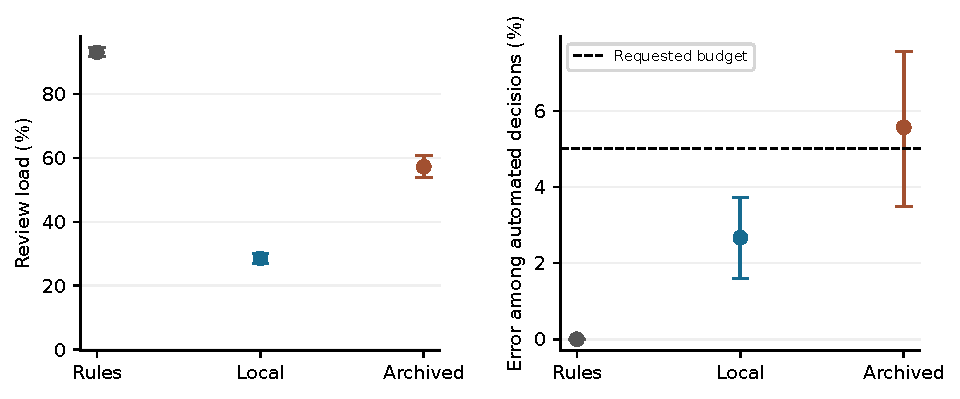
\includegraphics[width=.9\textwidth]{figures/v1_policy}
\caption{Review and automation error for locked 5\%-budget policies. Intervals
are conditional group-bootstrap intervals, not deployment bounds. The rule
policy has a degenerate zero-error empirical bootstrap interval.}\label{fig:policy}
\end{figure*}
Zero observed rule errors do not guarantee zero population risk: resampling 73
correct decisions cannot create unseen failures. An independent-Bernoulli
Wilson reference has an upper endpoint near 5\%, but does not account for
contrast-group dependence. Neither interval is a deployment-risk certificate.
The result is a review-load advantage at a common requested budget with unequal
realized risks. The earlier rule-unreachable claim does not hold on v1.

\section{Human-Validation Pilot}
The pilot samples \PilotCases{} distinct test identities: four cases per language
and generator class, including two surname contradictions per language, using
seed 20261028. It is balanced rather than prevalence-representative. Initial
annotators receive independently ordered worksheets with opaque IDs, observed
serialization, claims and unchanged definitions. Generator labels, clean values
and predictions are hidden. Uncertain is an annotation status, not an NLI label.

Initial responses match on 59/60 cases including uncertain statuses. Annotator
A marks 30 uncertain and B marks 31. Both give definite NLI labels on only 29;
conditional agreement and Cohen's kappa are 1.00 on those 29. Neither initially
uses contradiction, making its one-vs-rest kappa undefined. Language-wise
conditional results appear in Table~\ref{tab:pilot}. Perfect conditional kappa
does not establish reliable annotation across all 60 cases.

Initial adjudication covers 34 cases: the uncertainty union and three
definite-consensus disagreements with the generator. Follow-up reviews cover
the 11 still-blank cases and two human--generator disputes. The final two
reviewers agree on six entailments, four contradictions and three blank statuses.
Revisions and issue-specific feedback occurred; follow-up agreement is not a
fresh replication of the initial annotation study.

The reconciled record contains \PilotCandidates{} candidate human labels,
\PilotUnresolved{} unresolved cases and \PilotDisputes{} human--generator
disagreement. Unresolved cases concern a missing birth-date digit, ambiguous
expiry year and damaged date interval. Both follow-up reviewers reject a
surname variant accepted by the generator. We retain that disagreement without
relabeling frozen v1 or rescoring models. Some agreed rationales reconstruct
damaged text without unique support; consensus does not prove correctness.

Competence, independence and blinding declarations were received for A/B and
both follow-up reviewers. These are self-declarations, not independently
authenticated identities, qualifications or signatures. Personal attestations
and reviewer names are excluded from the anonymous submission.

\section{Discussion and Conclusion}
KYC-NLI distinguishes unsupported claims from uncertain automation. On frozen
moderate-noise v1, local XLM-R requires less review than rules at a common
requested error budget; archived XLM-R misses that empirical target. The result
depends on checkpoint identity and generator labels. Traceable artifacts and
human disagreement reporting are therefore part of the evidence. Generalization
to real documents, other noise conditions and independently validated labels
remains to be established.

\section*{Limitations}
\paragraph{Synthetic scope and labels.}
This evaluation uses one simulator, one moderate-noise condition and small name
pools. The negative-sampling repair covers engine and pool aliases, not all
linguistic equivalents. Neutral construction leaves detectable surface cues.
The selected pilot is small and partly unresolved; its candidate labels are not
replacement gold. It exposes tension between latent document truth and what
readers can establish from damaged observations. Existing semantics are retained,
not retroactively changed to favor either system.
\paragraph{Recovered models and retrospective analysis.}
Original training execution provenance is incomplete. The checkpoints are not
independent seeds; we report no training variance or causal explanation of their
gap. Test classification preceded selective analysis. Conditional intervals do
not cover policy selection, label uncertainty or distribution shift. No
deployment guarantee or new noise-generalization claim follows.
\paragraph{Human process.}
Initial uncertainty is extensive. Selected follow-up agreement does not repair
that measurement or verify independence. Revisions may introduce shared
interpretive influences. Prospective qualified language panels and adjudicated
OCR-reconstruction guidance remain necessary.

\section*{Ethics and Data Availability}
Benchmark identities are synthetic, not real identity records. Reviewer
declarations contain personal information and are kept private. We make no
blanket legal assertion about collecting real document corpora; authorization,
consent and governance require separate assessment. This diagnostic study must
not justify automatic customer rejection. Actual applications require
prospective evaluation of language-specific error and review burdens.

We plan to release code and synthetic data subject to licensing review.
Third-party resources retain their terms: Dakshina's distributor specifies
CC BY-SA 4.0, not a blanket license for every component or derived artifact.
No public release has occurred in this revision. The anonymous inventory
excludes private attestations, external corpora and model weights.

\bibliography{references}
\clearpage
\onecolumn
\appendix
\section{Additional Results and Artifact Identification}
\noindent\begin{minipage}[t]{.45\textwidth}
\centering\small% GENERATED by kyc-nli paper-v1; do not hand-edit.
\begin{tabular}{lrrr}
\toprule
System & E F1 & C F1 & N F1 \\
\midrule
Exact match & 0.193 & 0.613 & 0.000 \\
Rules & 0.550 & 0.646 & 0.622 \\
Local XLM-R & 0.966 & 0.978 & 1.000 \\
Archived XLM-R & 0.756 & 0.777 & 1.000 \\
\bottomrule
\end{tabular}

\captionof{table}{Class-wise F1 against generator labels.}
\end{minipage}\hfill
\begin{minipage}[t]{.51\textwidth}
\centering\small\resizebox{\linewidth}{!}{% GENERATED by kyc-nli paper-v1; do not hand-edit.
\begin{tabular}{ll}
\toprule
Comparison & Paired macro-F1 difference [95\% CI] \\
\midrule
Local XLM-R minus rules & 0.375 [0.336, 0.414] \\
Archived XLM-R minus rules & 0.238 [0.189, 0.290] \\
\bottomrule
\end{tabular}
}
\captionof{table}{Paired group-bootstrap macro-F1 differences.}\label{tab:paired}
\end{minipage}
\par\bigskip
\noindent\begin{minipage}[t]{.49\textwidth}
\centering\small\resizebox{\linewidth}{!}{% GENERATED by scripts/make_tables.py -- do not edit by hand.
% Regenerate the result, then re-run the script.
\begin{tabular}{lccccc}
\toprule
System & English & Hindi & Tamil & Bengali & Urdu \\
\midrule
Rule engine & 0.618 & 0.608 & 0.601 & 0.615 & 0.559 \\
Cross-encoder (ours) & 0.981 & 0.981 & 0.972 & 0.977 & 0.949 \\
\bottomrule
\end{tabular}
}
\captionof{table}{Language-wise macro-F1 with 95\% contrast-group bootstrap intervals.}
\end{minipage}\hfill
\begin{minipage}[t]{.47\textwidth}
\centering\small\resizebox{\linewidth}{!}{% GENERATED by kyc-nli paper-v1; do not hand-edit.
\begin{tabular}{lrrr}
\toprule
Language & Initial pairs & Definite pairs & Conditional kappa \\
\midrule
Bengali & 12 & 7 & 1.00 \\
English & 12 & 6 & 1.00 \\
Hindi & 12 & 5 & 1.00 \\
Tamil & 12 & 6 & 1.00 \\
Urdu & 12 & 5 & 1.00 \\
\bottomrule
\end{tabular}
}
\captionof{table}{Initial A/B agreement conditional on both responses being definite.}\label{tab:pilot}
\medskip
\begin{tabular}{ll}\toprule
Artifact & SHA-256 prefix \\\midrule
Local weights & \texttt{ae040c211cd2} \\
Archived weights & \texttt{469c1d7860f0} \\
Shared tokenizer & \texttt{17463f5db207} \\
Frozen v1 test & \texttt{10ef67fe3247} \\\bottomrule
\end{tabular}
\captionof{table}{Artifact prefixes; the inventory supplies full hashes.}\label{tab:hashes}
\medskip\raggedright
The evaluation records base revision \texttt{382f52958e59} plus an accompanying
source snapshot with local changes. Revision alone is not a complete experiment
identifier. Each frozen evaluation is separately inventoried. Paper outputs
come from pinned result hashes; historical caches are never fallback sources.
\end{minipage}
\par\bigskip
\begin{center}
\small\resizebox{\textwidth}{!}{% GENERATED by kyc-nli paper-v1; do not hand-edit.
\begin{tabular}{lrrrr}
\toprule
Phenomenon & Exact match & Rules & Local XLM-R & Archived XLM-R \\
\midrule
cross\_script\_name\_alt\_romanisation & 0.107 & 0.518 & 0.839 & 1.000 \\
cross\_script\_name\_icao & 0.277 & 0.755 & 0.947 & 0.936 \\
cross\_script\_name\_mismatch & 1.000 & 0.980 & 0.960 & 0.053 \\
date\_off\_by\_one & 1.000 & 0.253 & 1.000 & 1.000 \\
field\_absent\_from\_document & 0.000 & 1.000 & 1.000 & 1.000 \\
field\_illegible & 0.000 & 1.000 & 1.000 & 1.000 \\
impossible\_date\_triple & 1.000 & 0.287 & 1.000 & 0.973 \\
temporal\_consistent & 0.000 & 0.120 & 1.000 & 0.847 \\
\bottomrule
\end{tabular}
}
\captionof{table}{Accuracy by generator phenomenon, not a separate human-labelled test.}
\end{center}
\end{document}
